\chapter{Diagramas BPMN}\label{chap:bpmn-appendix}

\section{Introdução}

Os diagramas de Modelo e Notação de Processos de Negócio (Business Process Model and Notation - BPMN) servem para modelar um processo de negócio de maneira a unificar a visão sobre aquele processo e encontrar possíveis otimizações para o mesmo processo, evidenciando os pontos onde um futuro sistema pode agir.

\section{Processo antes do Sistema}

Os diagramas BPMN foram gerados com base nas entrevistas realizadas durante o processo de levantamento de requisitos. Vale lembrar que eles foram divididos de maneira a facilitar a visualização neste documento.

As figuras \ref{fig:bpmn-tcc1-pt1} e \ref{fig:bpmn-tcc1-pt2} mostram a modelagem BPMN para a disciplina de TCC1.

Já as figuras \ref{fig:bpmn-tcc2-pt1} e \ref{fig:bpmn-tcc2-pt2} mostram a modelagem BPMN para a disciplina de TCC2, porém desconsiderando os eventos de feira prática e banca teórica, para reduzir a complexidade e facilitar a visualização.

As figuras \ref{fig:bpmn-banca-feira-pt1} e \ref{fig:bpmn-banca-feira-pt2} mostram a modelagem BPMN os eventos de feira prática e banca teórica, responsáveis pela etapa final da disciplina de TCC2. A parte de recuperação de TCC2 foi desconsiderada nessas figuras, também para facilitar a visualização.

Por fim, para o processo de recuperação, foram modelados os diagramas das figuras \ref{fig:bpmn-rec-pt1} e \ref{fig:bpmn-rec-pt2}, que encerram o fluxo completo da disciplina de TCC2.

\begin{figure}[H]
    \centering
    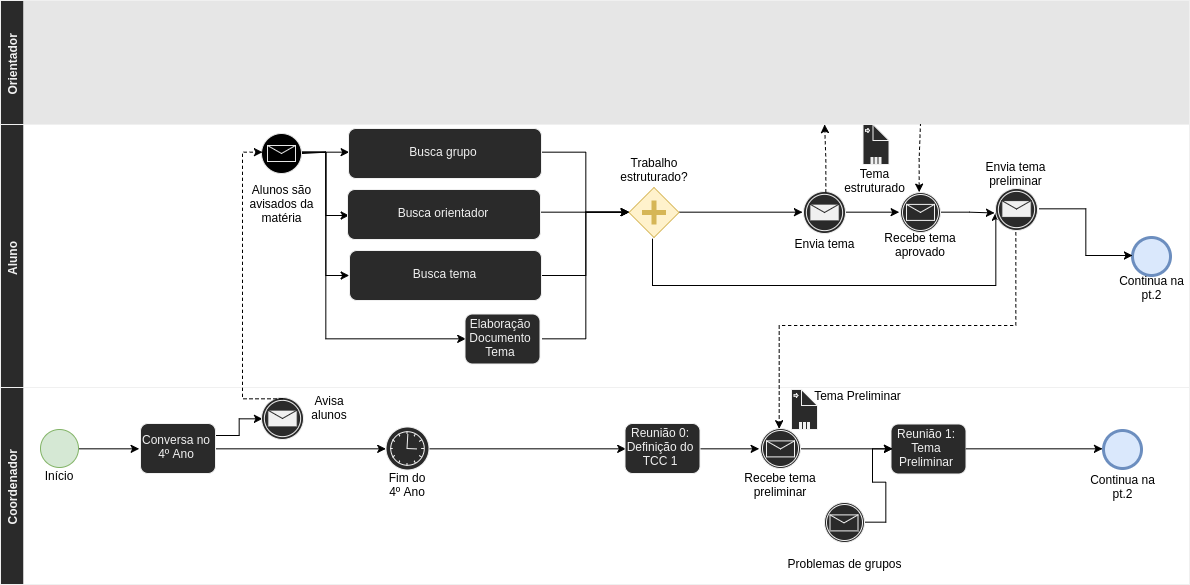
\includegraphics[angle=90, origin=c, scale=0.50]{bpmn-tcc1-pt1.png}
    \caption{Diagrama BPMN para a disciplina de TCC 1 - Parte 1}
    \label{fig:bpmn-tcc1-pt1}
\end{figure}

\begin{figure}[H]
    \centering
    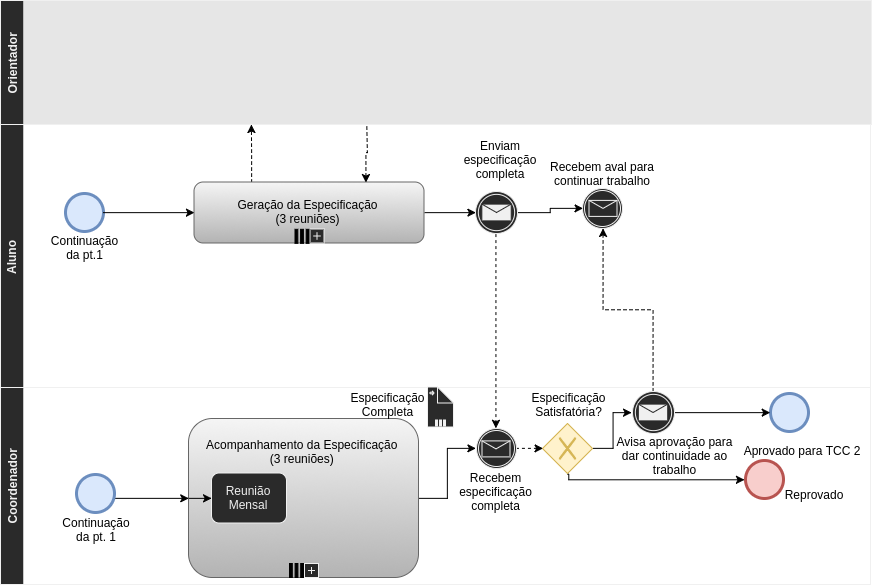
\includegraphics[angle=90, origin=c, scale=0.70]{bpmn-tcc1-pt2.png}
    \caption{Diagrama BPMN para a disciplina de TCC 1 - Parte 2}
    \label{fig:bpmn-tcc1-pt2}
\end{figure}

\begin{figure}[H]
    \centering
    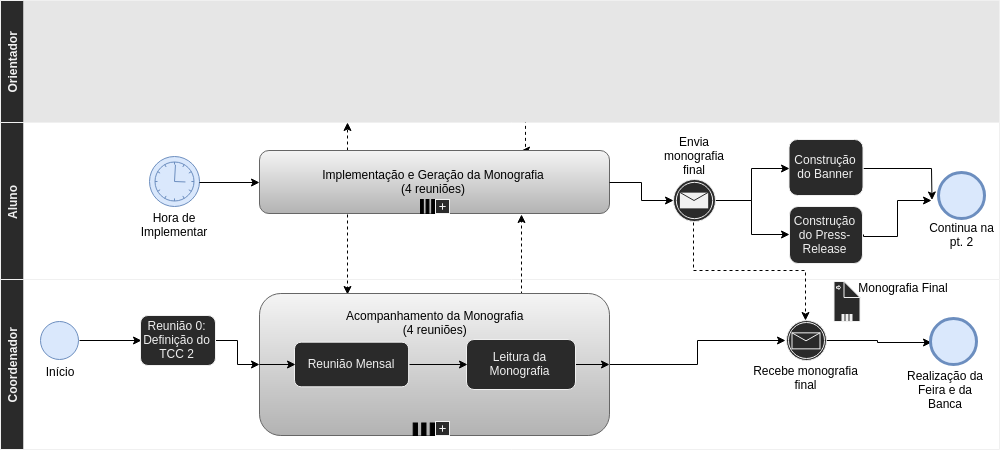
\includegraphics[angle=90, origin=c, scale=0.60]{bpmn-tcc2-pt1.png}
    \caption{Diagrama BPMN para a disciplina de TCC 2 - Parte 1}
    \label{fig:bpmn-tcc2-pt1}
\end{figure}

\begin{figure}[H]
    \centering
    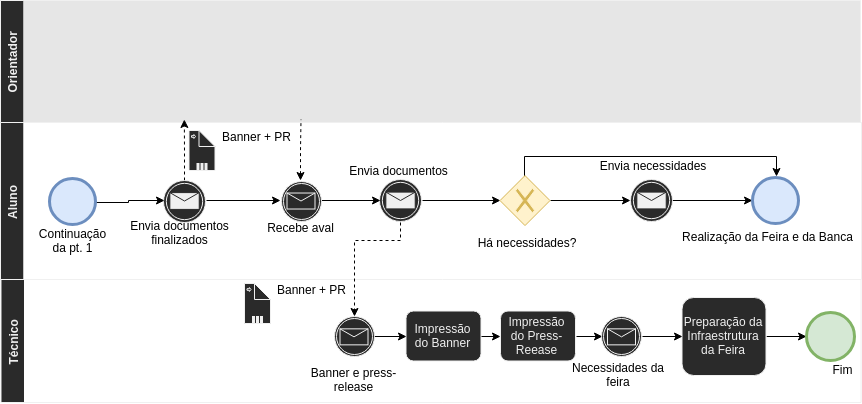
\includegraphics[angle=90, origin=c, scale=0.70]{bpmn-tcc2-pt2.png}
    \caption{Diagrama BPMN para a disciplina de TCC 2 - Parte 2}
    \label{fig:bpmn-tcc2-pt2}
\end{figure}

\begin{figure}[H]
    \centering
    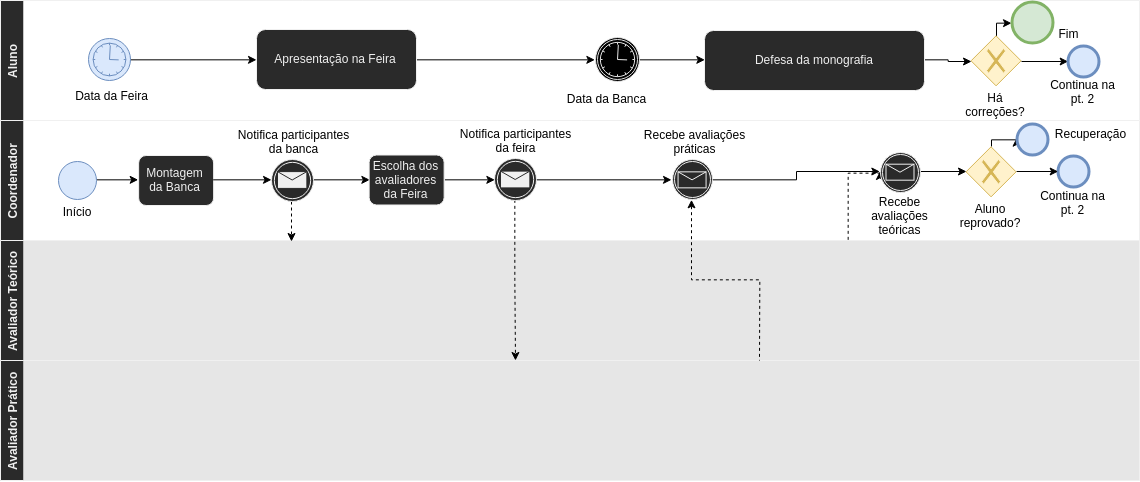
\includegraphics[angle=90, origin=c, scale=0.55]{bpmn-banca-feira-pt1.png}
    \caption{Diagrama BPMN para a Banca e Feira - Parte 1}
    \label{fig:bpmn-banca-feira-pt1}
\end{figure}

\begin{figure}[H]
    \centering
    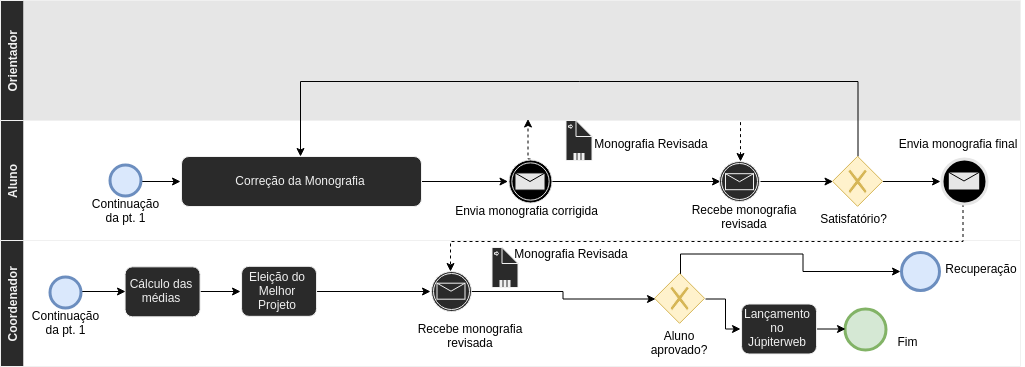
\includegraphics[angle=90, origin=c, scale=0.60]{bpmn-banca-feira-pt2.png}
    \caption{Diagrama BPMN para a Banca e Feira - Parte 2}
    \label{fig:bpmn-banca-feira-pt2}
\end{figure}

\begin{figure}[H]
    \centering
    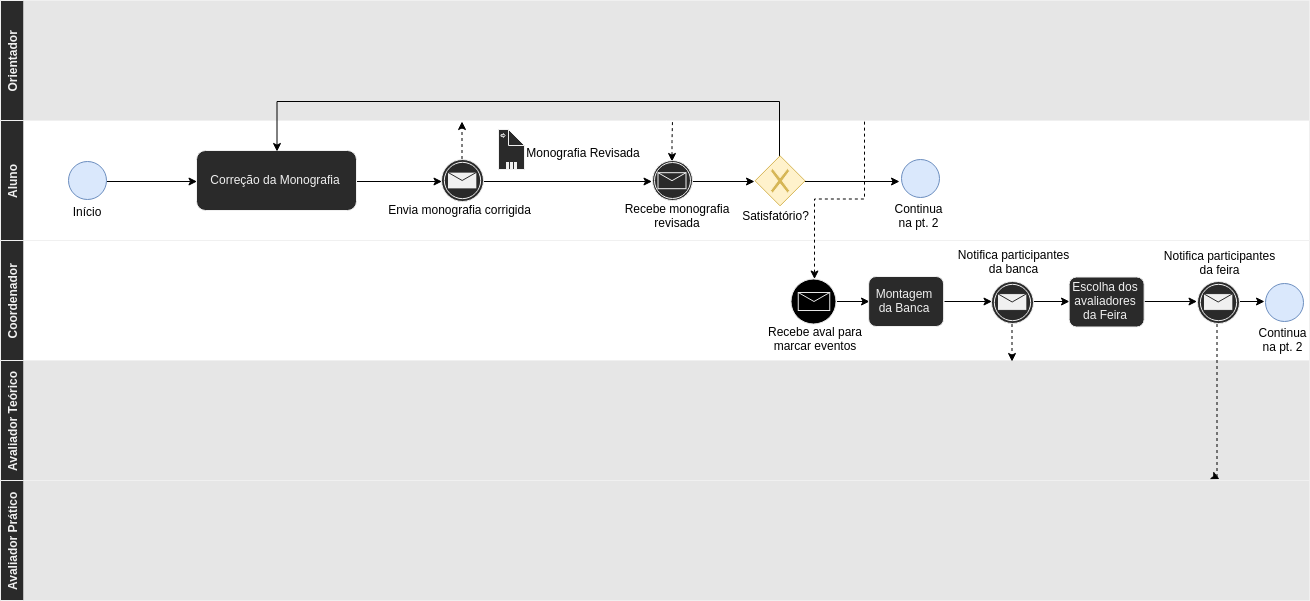
\includegraphics[angle=90, origin=c, scale=0.45]{bpmn-rec-pt1.png}
    \caption{Diagrama BPMN para a Recuperação - Parte 1}
    \label{fig:bpmn-rec-pt1}
\end{figure}

\begin{figure}[H]
    \centering
    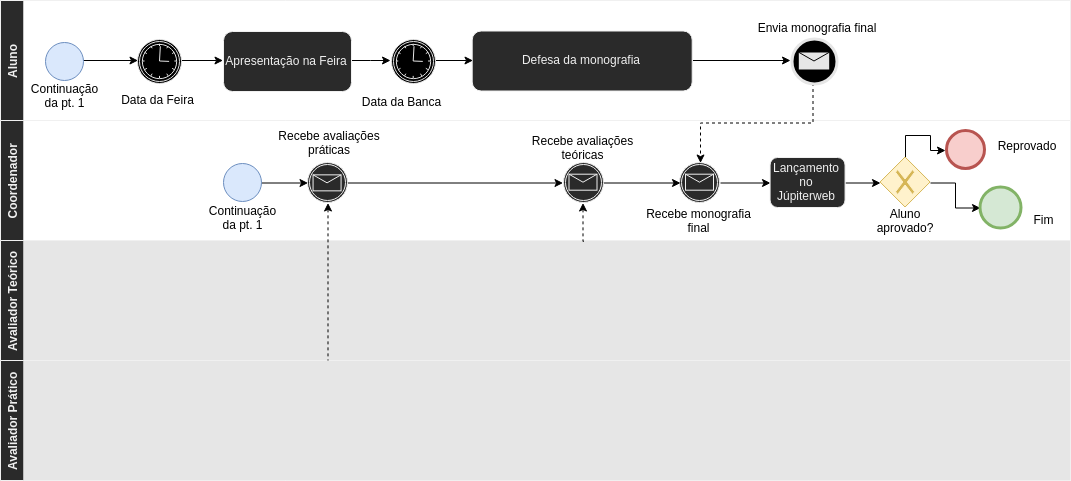
\includegraphics[angle=90, origin=c, scale=0.60]{bpmn-rec-pt2.png}
    \caption{Diagrama BPMN para a Recuperação - Parte 2}
    \label{fig:bpmn-rec-pt2}
\end{figure}
